% !TEX root = ../main.tex
\section{Method}

\subsection{Design}

\begin{table}
\begin{adjustbox}{width=\columnwidth}
\small
\begin{tabular}{llll}
\hline
\textbf{Name}      & \textbf{Short} & \textbf{Sequence}                                           & \textbf{Length} \\
\hline
T7 promoter        & 0          & GGTAATACGACTCACTATAG                                           & 20     \\
Short 1            & 1          & CCTCAAGGAGCTTCAGTCTAGCCCTATAGTGAGTCGTATTACC                    & 43     \\
Short 2            & 2          & CTCCTTGAGGCACATAACTCCCCTATAGTGAGTCGTATTACC                     & 42     \\
Short 3            & 3          & CACATAACTCTACTAAATCTCCCTATAGTGAGTCGTATTACC                     & 42     \\
Short 4            & 4          & CACATAACTCTACTAAATCTCCCTATAGTGAGTCGTATTACC                     & 42     \\
Short 5            & 5          & AGATTTAGTAGAGTTATGTGCCCTATAGTGAGTCGTATTACC                     & 42     \\
Long 1             & 6          & GTCAATTCGCCTCAAGGAGCTTCAGTCTAGCCCTATAGTGAGTCGTATTACC           & 52     \\
Long 2             & 7          & GCTCCTTGAGGCGAATTGACCCATCTTCATTCTACTCCTACCCTATAGTGAGTCGTATTACC & 62     \\
Long 3             & 8          & CCATCTTCATTCTACTCCTATACCTCAATCCCCTATAGTGAGTCGTATTACC           & 52     \\
Long 4             & 9          & TAGGAGTAGAATGAAGATGGGTCAATTCGCCTCAAGGAGCCCCTATAGTGAGTCGTATTACC & 62     \\
Long 5             & 10         & GATTGAGGTATAGGAGTAGAATGAAGATGGCCCTATAGTGAGTCGTATTACC           & 52     \\
% Beacon fluorophore & 11         & CGGCTAGACTGAA                                                  & 13     \\
% Beacon quencher    & 12         & CCTCAAGGAGCTTCAGTCTAGCCG                                       & 24 \\
\hline
\end{tabular}
\end{adjustbox}
\caption{Sequences and names of the DNA strands used for transcription.}
\end{table}

\begin{table}
\begin{adjustbox}{width=\columnwidth}
\small
\begin{tabular}{llll}
\hline
\textbf{Name}      & \textbf{Short} & \textbf{Sequence}                                           & \textbf{Length} \\
\hline
Short 1            & 1          & GGCUAGACUGAAGCUCCUUGAGG                    & 23     \\
Short 2            & 2          & GGGAGUUAUGUGCCUCAAGGAG                     & 22     \\
Short 3            & 3          & GGAGAUUUAGUAGAGUUAUGUG                     & 22     \\
Short 4            & 4          & GGCUCCUUGAGGCACAUAACUC                     & 22     \\
Short 5            & 5          & GGCACAUAACUCUACUAAAUCU                     & 22     \\
Long 1             & 6          & GGCUAGACUGAAGCUCCUUGAGGCGAAUUGAC           & 32     \\
Long 2             & 7          & GGUAGGAGUAGAAUGAAGAUGGGUCAAUUCGCCUCAAGGAGC & 42     \\
Long 3             & 8          & GGGAUUGAGGUAUAGGAGUAGAAUGAAGAUGG           & 32     \\
Long 4             & 9          & GGGCUCCUUGAGGCGAAUUGACCCAUCUUCAUUCUACUCCUA & 42     \\
Long 5             & 10         & GGCCAUCUUCAUUCUACUCCUAUACCUCAAUC           & 32     \\
% Beacon fluorophore & 11         & CGGCTAGACTGAA                                                  & 13     \\
% Beacon quencher    & 12         & CCTCAAGGAGCTTCAGTCTAGCCG                                       & 24 \\
\hline
\end{tabular}
\end{adjustbox}
\caption{Sequences and names of the transcribed RNA strands.}
\end{table}

\subsection{Transcription}

The oligos from IDT was dissolved in TE buffer [PROTOCOL] to an approximate concentration of 120 $\mu$M, based on the quantity of substance written on the tubes. The final concentration desired was 100 $\mu$M, but due to a risk of inaccurate substance quantities, the dissolved concentration was chosen to be slightly above. The oligos could then be further diluted after measuring their absorbance on the Nanodrop.

After dissolving the oligos, the absorbance of each sample was measured on the Nanodrop in triplets. A program was written which can take the .csv output of the Nanodrop, and calculate the concentration based on each strands extinction coefficient \cite{nanodropimport}.

The measured concentrations (figure \ref{oligo_concentrations}) was used to dilute the samples further, to a concentration of 100 $\mu$M.

To anneal the templates to the promoter, each of the template strands was mixed with equal amounts of promoter strand in annealing buffer [PROTOCOL], to a final concentration of 1 $\mu$M. The mixed samples were then heated to 90$^\circ$ C for 5 minutes, and left to cool down to room temperature.

To check if samples annealed properly, they were run on a 20\% native PAGE gel for 3 hours. Each lane was loaded with 50 $\mu$l sample, and 10 $\mu$l native loading buffer [PROTOCOL]. Afterwards the gel was stained in SYBR Gold, and visualised on the Typhoon scanner [PROTOCOL]. The result of the scan can be seen in figure \ref{fig:promoter_annealing_gel}.

\begin{figure}[H]
\centering
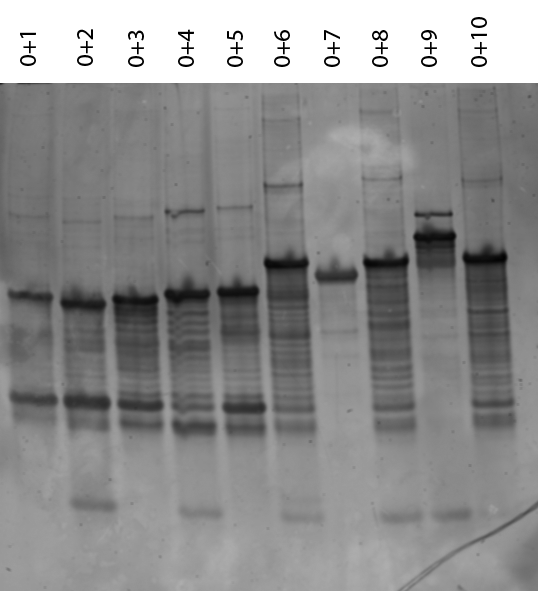
\includegraphics[width=\columnwidth]{images/promoter_annealing_gel.png}
\caption{Typhoon scan of SYBR Gold stained native PAGE gel, with the annealed templates and promoter strands. The lanes are labelled by which strands are annealed (see table [CREATE TABLE WITH NAMES OF STRANDS]).}
\label{fig:promoter_annealing_gel}
\end{figure}

As can be seen in figure \ref{fig:promoter_annealing_gel}, the darkest bands is the annealed samples. The samples for the short translator runs as about the same size, while there is bigger variation in the long translator samples, as expected based on [TABLE WITH STRANDS]. The exact positions of the long translator samples does not match with the sequence length, though this can be explained by secondary structures of the single-stranded part of the sample. The shorter bands visible below, is probably surplus promoter, other secondary structures, and shorter sequences from synthesis errors.
